\chapter[Requirements, Design, and Implementation]{Requirements, Design, And\\ Implementation}\label{ch:ReqDesignImp}
\section{Requirements}
As we have previously mentioned, the role of our team's project positions us squarely between the the Collection Management team and the Solr team when discussing the overall workflow of the system. Based upon group discussions in a classroom setting, it was decided what information that the Collection Management team would provide to the other teams that need to work with cleaned tweet data. A full specification of these decisions can be found by viewing the Collection Management team's report, however we will briefly discuss the points that were relevant to us.

Given the cleaned tweet data from Collection Management, we our team will then be able to perform the methodologies we describe later to classify whether a document is relevant or irrelevant to a given class. A detailed layout of the project with our interactions highlighted is provided by Figure \ref{fig:design}.

We will then place our classification information in the HBase datastore to mark the relevance of each document. The Solr team will then index this class information that we provide, allowing for more robust query results and more useful facets to be created.

\begin{figure}[ht]
	\centering
	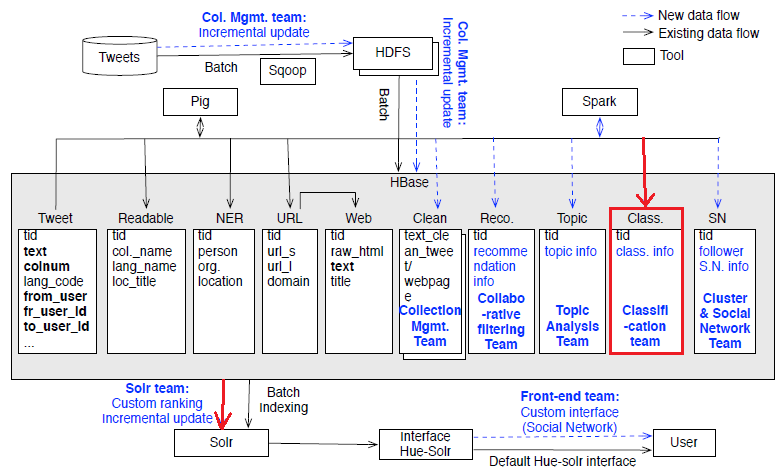
\includegraphics[width=\textwidth]{figures/data_flow.png}
    \caption{Layout of the project teams, as provided by Professor Fox and his GRAs.}\label{fig:design}
\end{figure}

\section{Design}
Our current design is based primarily off of recommendations from the GRAs assisting the class. We have also taken substantial input from last year's Classification team \cite{cui2015classification} and the Professor.

We have designed our current solution around pulling training data from and testing on a small collection of around 100,000 tweets. This was originally going to be performed on the small collection that was assigned to our team, \texttt{\#germanwings}. However, due to some changes and discussion among the other teams, we have decided to continue with designing and testing our solution using a cleaned dataset provided by the Collection Management team. However this dataset was not made available until after our current solution was mostly implemented using our original small dataset. Therefore for the rest of this document we will be using the small dataset \texttt{z\_602}, \texttt{\#germanwings}. All future work will be done using cleaned data from the collection management team.

\begin{figure}[ht]
	\centering
	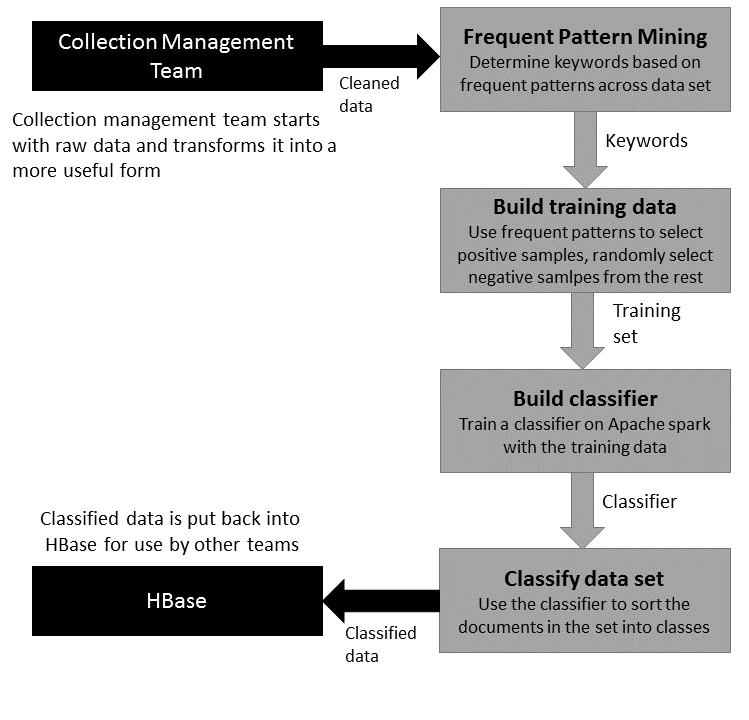
\includegraphics[scale=.65]{figures/design_flow_chart.png}
    \caption{High level overview of the flow of data through the system.}\label{fig:overview}
\end{figure}

\section{Implementation}
Our implementation can be easily laid out in a step by step workflow, with only one step requiring true manual input and evaluation from a person. Below we will discuss each step in detail.

Our methodology primarily revolves around building a training set. This training set will be used for training a machine learning model, a.k.a.\ a classifier.

\subsection{Environment Set--Up}
Our group decided to avoid working directly on the cluster to allow us full administrative rights to a machine, allowing us to set up and test different configurations and algorithms than what might currently be supported by the Hadoop cluster being used for class.

A prime example, and the primary motivating factor for our choice was our decision to use Frequent Pattern Mining (FPM) in the construction of our training sets. The cluster provided for the class is currently running Spark version 1.2.0, FPM is not supported by Spark until version 1.5.0. Since FPM was a methodology suggested by the GRAs, and they assured us that they could upgrade the cluster to a more current version of Spark, we decided to proceed with this method.

Due to time constraints, we created a Debian Virtual Machine with sufficient specs to begin writing and testing our methodology. This machine is hosted on a VMware vSphere cluster and has been assigned 32 GB of RAM, 16 processor cores, and 40 GB of storage. This has proven to be more than adequate for the testing that we have performed on our small data set.

As of the time of this writing, we are still waiting for the GRAs to upgrade the Spark instance on the full cluster, allowing us and the the other groups to make full use of our methods.

\subsection{Building the Training Data}
In order to begin the classification process we have to pull out and determine a set of training data to use for the machine learning classification algorithm. In order to do this, we assume that we are working with data that has been cleaned of profanity and non-printable characters.

For our methodology we then need to take the content of each tweet as a string and tokenize it. This means that we will remove any duplicate words and have the result be a set of the vocabulary in the tweet. At this stage we also remove any stop words that are in the vocabulary to make sure our algorithms in the next phase are not skewed by taking stop words into account. During this phase we also strip the \# from any hashtags that are present in the tweet.

In our initial design and testing we did not yet have access to cleaned tweets from the collection management team, so we worked primarily to build the methodology that would be used once those tweets became available. Therefore some of the steps mentioned previously, such as the removal of the stop words and the removal of the \# from hashtags are unnecessary when working with the data provided by Collection Management in HBase.

The next step in our algorithm involves the use of Frequent Pattern Mining (FPM) to determine the most frequently used patterns of words in the tweet text. FPM looks at the set of existing vocabulary for each text and determines which tokens appear together within a tweet's vocabulary most often.

This is the stage where manual intervention in necessary. We look at a file containing a sorted list of all the frequent patterns, from this we choose a set of features to train on. In our attempts at training a classifier for our small data collection, we chose to select a frequent pattern of four words. This was essentially an arbitrary choice, but we believe that it strikes a good balance between being too specific and missing some relevant tweets and being too broad and pulling in a number of irrelevant tweets.

At this stage we need to create positive and negative training samples. To do this, we pull a random subset of tweets that contain our frequent pattern and classify those as positive samples. For our negative sample we pull a random subset of tweets that do not contain our frequent pattern.

\subsection{Training the Classifier}

We then use the sets of positive and negative samples to train a classifier. We are currently using a logistic regression classifier in our implementation, primarily due to its ease of implementation in Spark.

As the project progresses we plan to attempt using several different classifiers and comparing their effectiveness at classifying our data.

\subsection{Predicting the Class}

After training the classifier, we apply the classifier to all the tweets across our small data collection. This results in a binary scoring for each tweet as relevant or irrelevant to the collection based upon the training data we selected.

We can evaluate the accuracy of our model by judging how well it classified some of the data that could have been in our positive or negative samples. We currently do not have this well implemented, but plan to have this evaluation completed before the next report.


% Here is the introduction. The next chapter is chapter~\ref{ch:ch2label}.


% a new paragraph


% \section{Examples}
% You can also have examples in your document such as in example~\ref{ex:simple_example}.
% \begin{example}{An Example of an Example}
%   \label{ex:simple_example}
%   Here is an example with some math
%   \begin{equation}
%     0 = \exp(i\pi)+1\ .
%   \end{equation}
%   You can adjust the colour and the line width in the {\tt macros.tex} file.
% \end{example}

% \section{How Does Sections, Subsections, and Subsections Look?}
% Well, like this
% \subsection{This is a Subsection}
% and this
% \subsubsection{This is a Subsubsection}
% and this.

% \paragraph{A Paragraph}
% You can also use paragraph titles which look like this.

% \subparagraph{A Subparagraph} Moreover, you can also use subparagraph titles which look like this\todo{Is it possible to add a subsubparagraph?}. They have a small indentation as opposed to the paragraph titles.

% \todo[inline,color=green]{I think that a summary of this exciting chapter should be added.}